
\documentclass{ctexart}
\usepackage{amsmath,bm}
\usepackage{setspace}
\usepackage{xeCJK}
\usepackage{xcolor}
\usepackage{indentfirst}
\usepackage{listings}
\usepackage{graphicx}
\usepackage{subfigure}
\usepackage{amsfonts,amssymb}
\usepackage[a4paper,scale=0.8]{geometry}
\usepackage{hyperref}
\usepackage{float}
\usepackage{changepage}
\usepackage{xcolor}
\usepackage{listings}
\usepackage{longtable}
\lstset{
basicstyle=\small,%
escapeinside=``,%
keywordstyle=\color{red} \bfseries,% \underbar,%
identifierstyle={},%
commentstyle=\color{blue},%
stringstyle=\ttfamily,%
%labelstyle=\tiny,%
extendedchars=false,%
linewidth=\textwidth,%
numbers=left,%
numberstyle=\tiny \color{blue},%
frame=trbl%
}

\newcommand{\tabincell}[2]{\begin{tabular}{@{}#1@{}}#2\end{tabular}}
\lstset{breaklines}%这条命令可以让LaTeX自动将长的代码行换行排版

\lstset{extendedchars=false}%这一条命令可以解决代码跨页时,章节标题,页眉等汉字不显示的问题
\setCJKmainfont{华光书宋_CNKI}
\newCJKfontfamily\kaiti{华光楷体_CNKI}
\newCJKfontfamily\hei{华光黑体_CNKI}
\newCJKfontfamily\fsong{华光仿宋_CNKI}
\newfontfamily\code{Courier New}
\linespread{1.5} \setlength\parindent{2 em}
\title{\Huge 中国科学技术大学计算机学院\\《计算机体系结构》实验报告}
\date{\LARGE 2021.06.07}
\begin{document}
\begin{hei}  \maketitle\end{hei}
\begin{figure}[htbp]
    \centering
    
\includegraphics[scale=0.4]{USTC.png}

\end{figure}
\begin{LARGE}\begin{align*}    & \text{实验题目:\underline{Tomasulo软件模拟器和多Cache一致性软件模拟器}} \\
         & \text{学生姓名:\underline{胡毅翔}}                                      \\
         & \text{学生学号:\underline{PB18000290}}\end{align*}\end{LARGE}
\par
\par\par
\centerline{\large 计算机实验教学中心制}
\par \centerline {\large 2019年9月}
\newpage
\section{\hei 实验目的}
\begin{enumerate}
    \item 熟悉Tomasulo模拟器和cache一致性模拟器(监听法和目录法)的使用。
    \item 加深对Tomasulo算法的理解,从而理解指令级并行的一种方式-动态指令调度。
    \item 掌握Tomasulo算法在指令流出、执行、写结果各阶段对浮点操作指令以及load和store指令进行什么处理;给定被执行代码片段,对于具体某个时钟周期,能够写出保留站、指令状态表以及浮点寄存器状态表内容的变化情况。
    \item 理解监听法和目录法的基本思想,加深对多cache一致性的理解。
    \item 做到给出指定的读写序列,可以模拟出读写过程中发生的替换、换出等操作,同时模拟出cache块的无效、共享和独占态的相互切换。
\end{enumerate}
\section{\hei 实验环境}
\begin{enumerate}

    \item PC一台
    \item Windows 10操作系统
    \item Vivado 2019.1
    \item Visual Studio Code 1.56.2
    \item Tomasulo模拟器
    \item 多Cache一致性模拟器

\end{enumerate}
\section{\hei Tomasulo算法模拟器}
使用模拟器进行以下指令流的执行并对模拟器截图、回答问题。
\begin{lstlisting}[language={[x86masm]Assembler}]
    L.D  F6, 21(R2)
    L.D  F2, 0(R3)
    MUL.D  F0, F2, F4
    SUB.D  F8, F6, F2
    DIV.D  F10, F0, F6
    ADD.D  F6, F8, F2
    \end{lstlisting}
\par 假设浮点功能部件的延迟时间:加减法2个周期,乘法10个周期,load/store2个周期,除法40个周期。
\begin{enumerate}
    \item 分别截图(当前周期2和当前周期3),请简要说明load部件做了什么改动。
          \par 周期2:Load部件:占用Load2部件,Busy置位;R2就绪,将地址保存在Load1部件的地址寄存器。
          \par \begin{figure}[htbp]
              \centering
              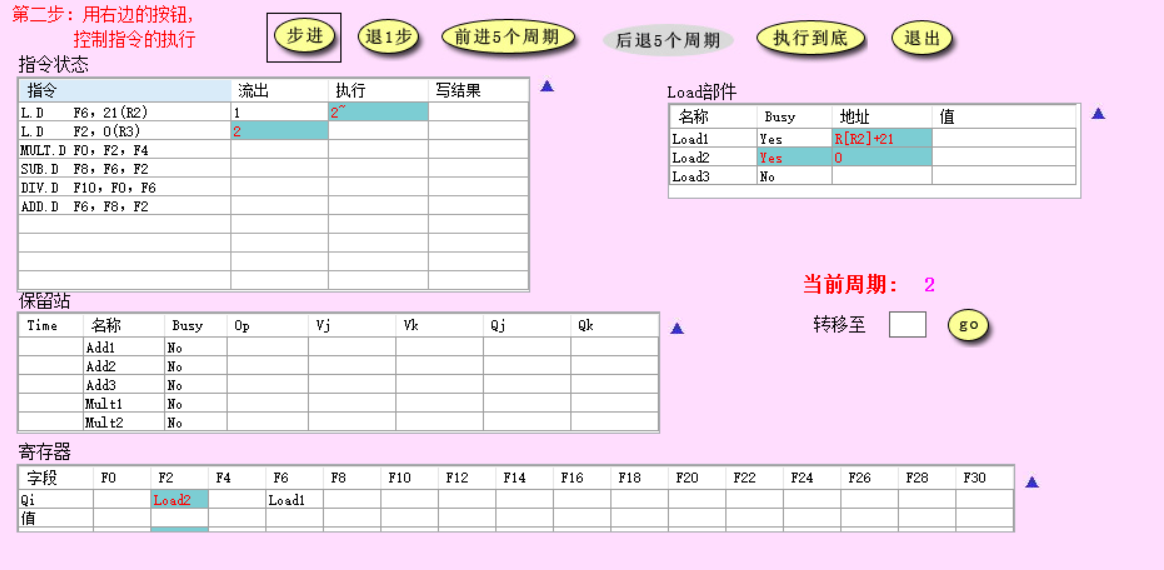
\includegraphics[scale=0.3]{zq2.png}
              \caption{周期2}
          \end{figure}
          \par 周期3:Load部件:Load1部件将从存储器读到的值保存在Load1部件寄存器;R3就绪,将地址保存在Load2部件地址寄存器。
          \par \begin{figure}[htbp]
              \centering
              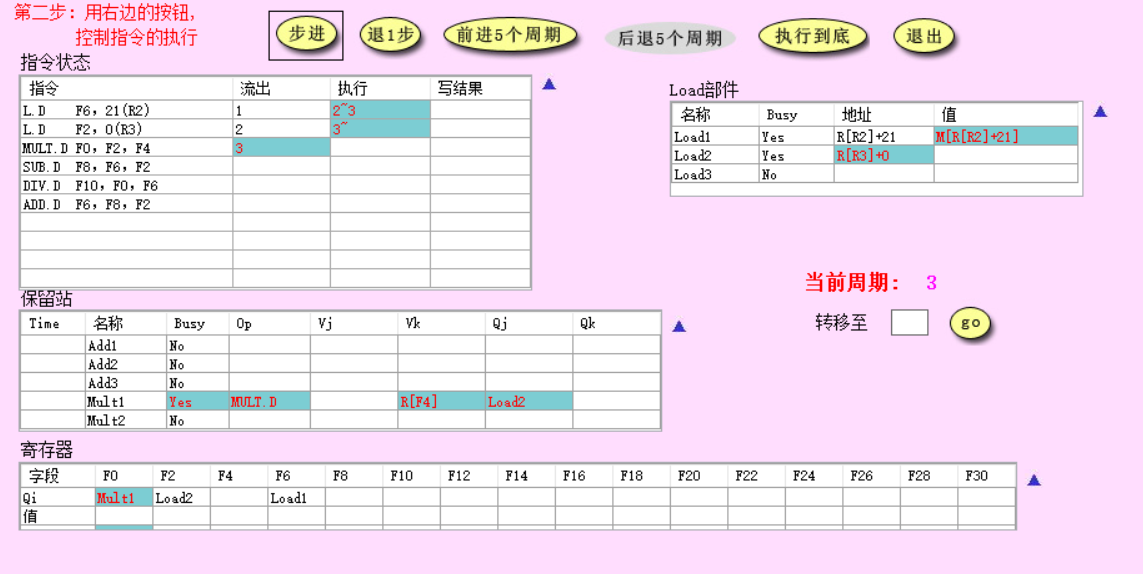
\includegraphics[scale=0.3]{zq3.png}
              \caption{周期3}
          \end{figure}
    \item 请截图(MUL.D刚开始执行时系统状态),并说明该周期相比上一周期整个系统发生了哪些改动(指令状态、保留站、寄存器和Load部件)。
          \par 相比上一周期系统发生的改变:
          \begin{itemize}
              \item 指令状态:发射第6条指令;第三条、第四条指令进入执行状态。
              \item Load部件:无变化。
              \item 保留站:新发射的ADD.D指令占用Add2保留站,进入执行的指令MUL.D和SUB.D开始执行,时间开始倒计时。
              \item 寄存器:新发射的指令ADD.D指令等待F8寄存器。
          \end{itemize}
          \par
          \begin{figure}[H]
              \centering
              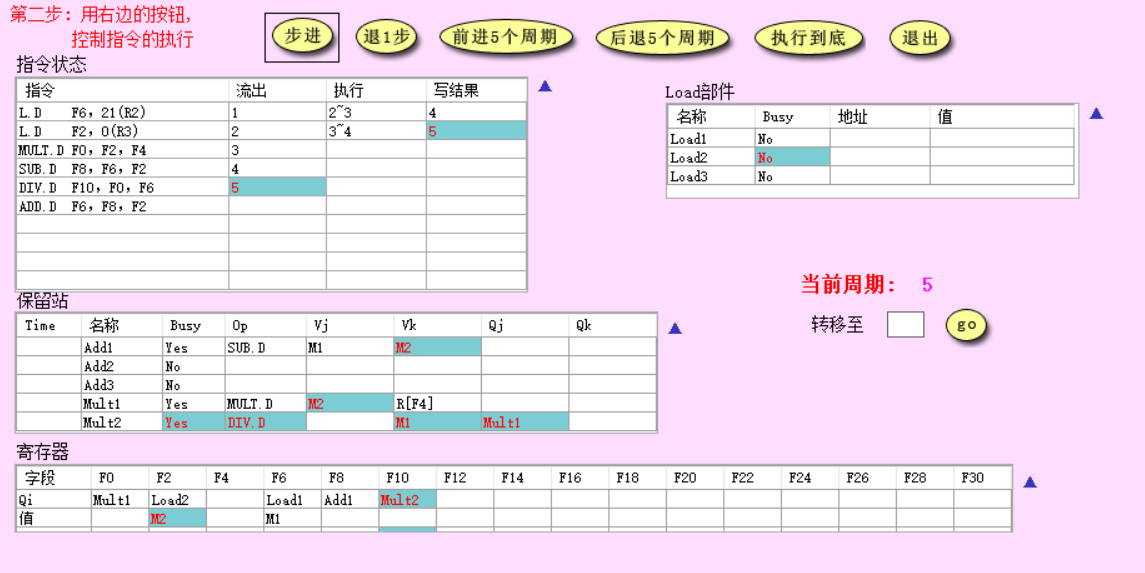
\includegraphics[scale=0.3]{zq5.png}
              \caption{周期5(上一周期)}
          \end{figure}
          \par \begin{figure}[H]
              \centering
              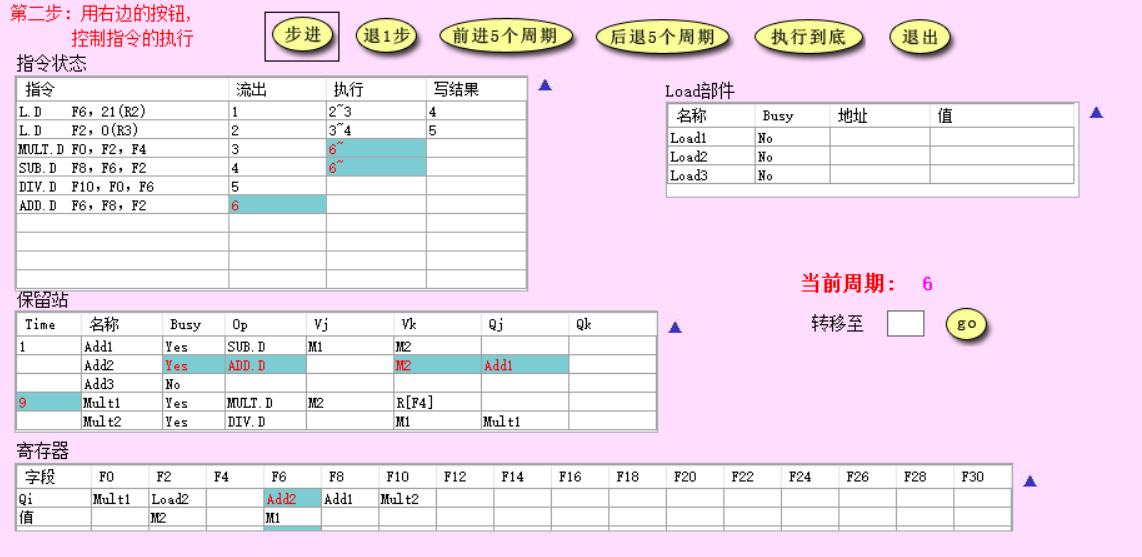
\includegraphics[scale=0.3]{zq6.png}
              \caption{周期6(MUL.D刚开始执行)}
          \end{figure}
    \item 简要说明是什么相关导致MUL.D流出后没有立即执行。
          \par 源操作数F2为写回,直到第五周期M2写入后才就绪。
    \item 请分别截图(15周期和16周期的系统状态),并分析系统发生了哪些变化。
          \par 周期15:指令ADD.D和指令SUB.D在周期7~15周期内执行完毕,将结果写回,释放相应的保留站和寄存器;此时MULT.D指令执行了10个周期。
          \begin{figure}[H]
              \centering
              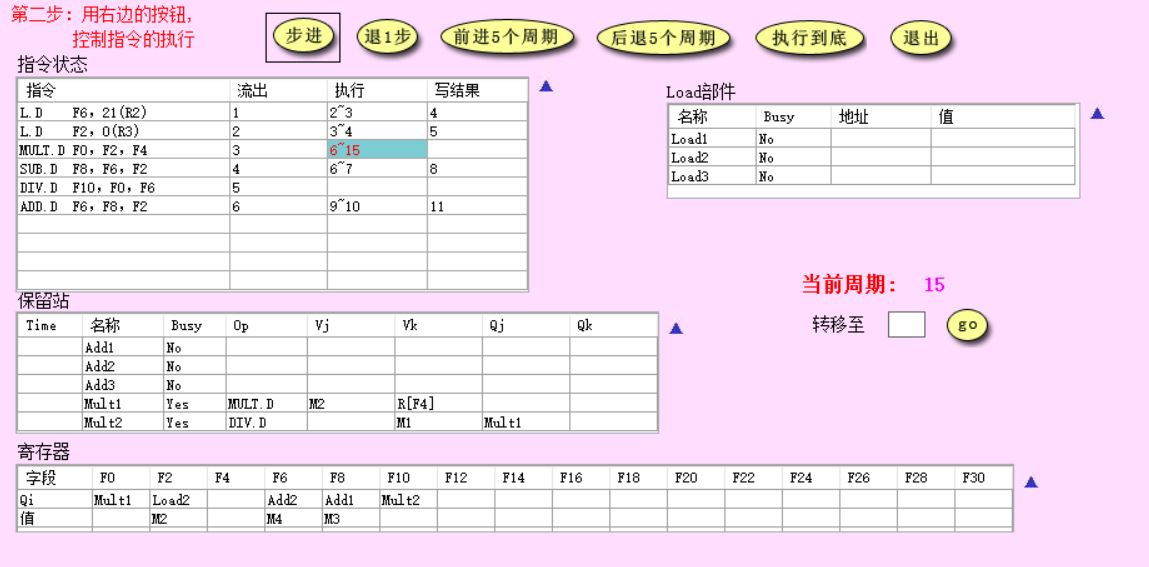
\includegraphics[scale=0.3]{zq15.png}
              \caption{周期15}
          \end{figure}
          \par 周期16:指令MUL.D写回结果,释放保留站CBD将结果广播到寄存器和指令DIV.D对应的保留站。
          \begin{figure}[H]
              \centering
              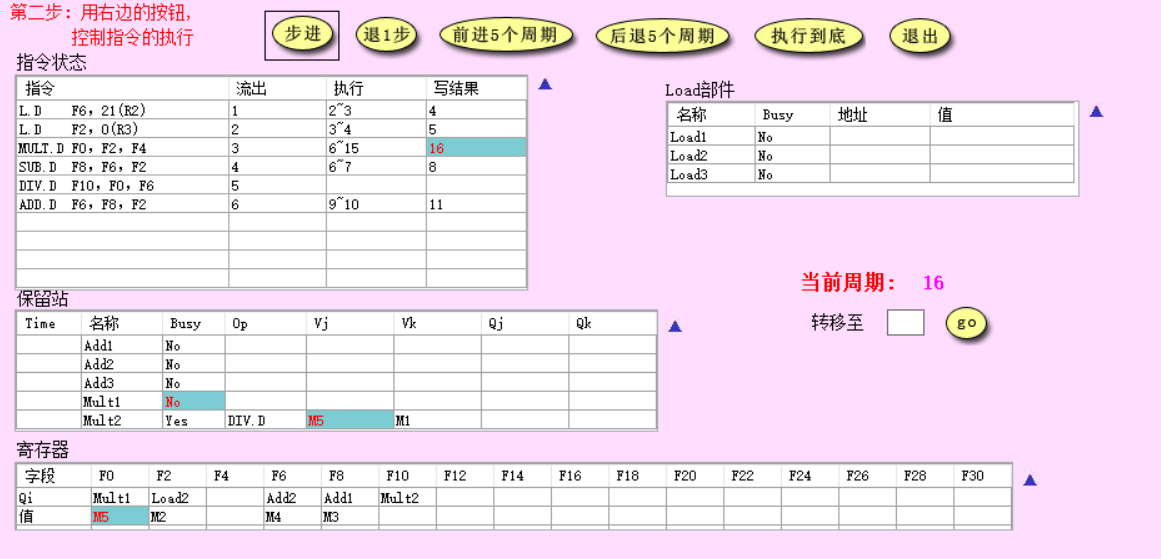
\includegraphics[scale=0.3]{zq16.png}
              \caption{周期16}
          \end{figure}
    \item 回答所有指令刚刚执行完毕时是第多少周期,同时请截图(最后一条指令写CBD时认为指令流执行结束)。
          \begin{figure}[H]
              \centering
              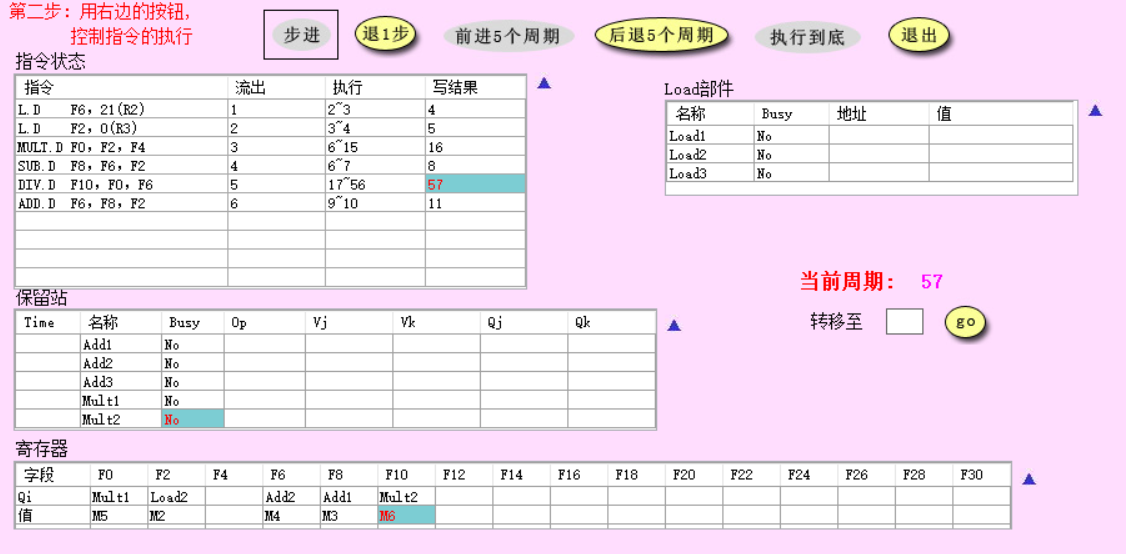
\includegraphics[scale=0.3]{zq57.png}
              \caption{周期57}
          \end{figure}
          \par
          所有指令执行完毕是第57个周期。
\end{enumerate}
\section{\hei 多cache一致性算法-监听法}
\begin{enumerate}
    \item 利用模拟器进行下述操作,并填写下表。
    \begin{longtable}{|l|l|l|l|}
        % \begin{longtable}{p{1cm}, p{1cm}, p{1cm}, p{1cm}}

        \caption{监听法}\label{tab1}

        % 表格“首页”显示内容

        \endfirsthead

        % “后续页面”表头显示内容
        \multicolumn{1}{c}{Continued}                   \\

        \endhead

        % 表格“尾页前”,表格最后显示内容

        \multicolumn{1}{c}{Continued on next page}
        \endfoot

        % 表格“尾页”,表格最后显示内容

        \endlastfoot
        \hline
        所进行的访问      & 是否发生了替换?     & 是否发生了写回?    & 监听协议进行的操作与块状态改变                                                                     \\ \hline
        CPU A 读第5块  & 替换Cache A的块1 & 0           & \tabincell{l}{CacheA发射Read Miss,\\存储器传输第5块到CacheB,\\CacheA的块1从状态I转为S}                                  \\ \hline
        CPU B 读第5块  & 替换CacheB的块1  & 0           & \tabincell{l}{CacheB发射Read Miss,\\存储器传输第五块到CacheB,\\CacheB的块1从状态I转为S}                                  \\ \hline
        CPU C 读第5块  & 替换CacheC的块1  & 0           & \tabincell{l}{CacheC发射Read Miss,\\存储器传输第5块到CacheC,\\CacheC的块1从状态I转换为S}                               \\ \hline
        CPU B 写第5块  & 0            & 0           & \tabincell{l}{CacheB发射Invalidate,\\CacheA的块1从状态S转换到I,\\CacheC的块1从状态S转换到I,\\CacheB的块1从S转换到M}              \\ \hline
        CPU D 读第5块  & 替换CacheD的块1  & CacheB的块1写回 & \tabincell{l}{CacheD发射Read Miss,\\CacheB写回第5块,\\存储器传输第5块到CacheD,\\CacheB的块1从状态M转换到S,\\CacheD的块从状态I转换到S}    \\ \hline
        CPU B 写第21块 & 替换CacheB的块1  & 0           & \tabincell{l}{CacheB发射Write Miss,\\存储器传输第21块到CacheB,\\CacheB的块1从状态S转换为M}                               \\ \hline
        CPU A 写第23块 & 替换CacheA的块3  & 0           & \tabincell{l}{CacheA发射Write Miss,\\存储器传输第23块到CacheA,\\CacheA的块1从状态I转换到M}                               \\ \hline
        CPU C 写第23块 & 替换CacheC的块3  & CacheA的块3写回 & \tabincell{l}{CacheC发射Read Miss,\\CacheA写回第23块,\\存储器传输第23块到CacheC,\\CacheA的块3从状态M转换到I,\\CacheC的块3从状态I转换到M} \\ \hline
        CPU B 读第29块 & 替换CacheB的块1  & CacheB的块1写回 & \tabincell{l}{CacheB写回第21块,\\CacheB发射Read Miss,\\存储器传输第29块到CacheB,\\CacheB的块1从状态M转换到S}                   \\ \hline
        CPU B 写第5块  & 替换CacheB的块1  & 0           & \tabincell{l}{CacheB发射Write Miss,\\存储器传输第5块到CacheB,\\CacheB的块1从状态S转换到M,\\CacheD的块1从状态S转换带I}              \\ \hline
    \end{longtable}
    \item 请截图,展示执行完以上操作后整个cache系统的状态。
          \par \begin{figure}[H]
              \centering
              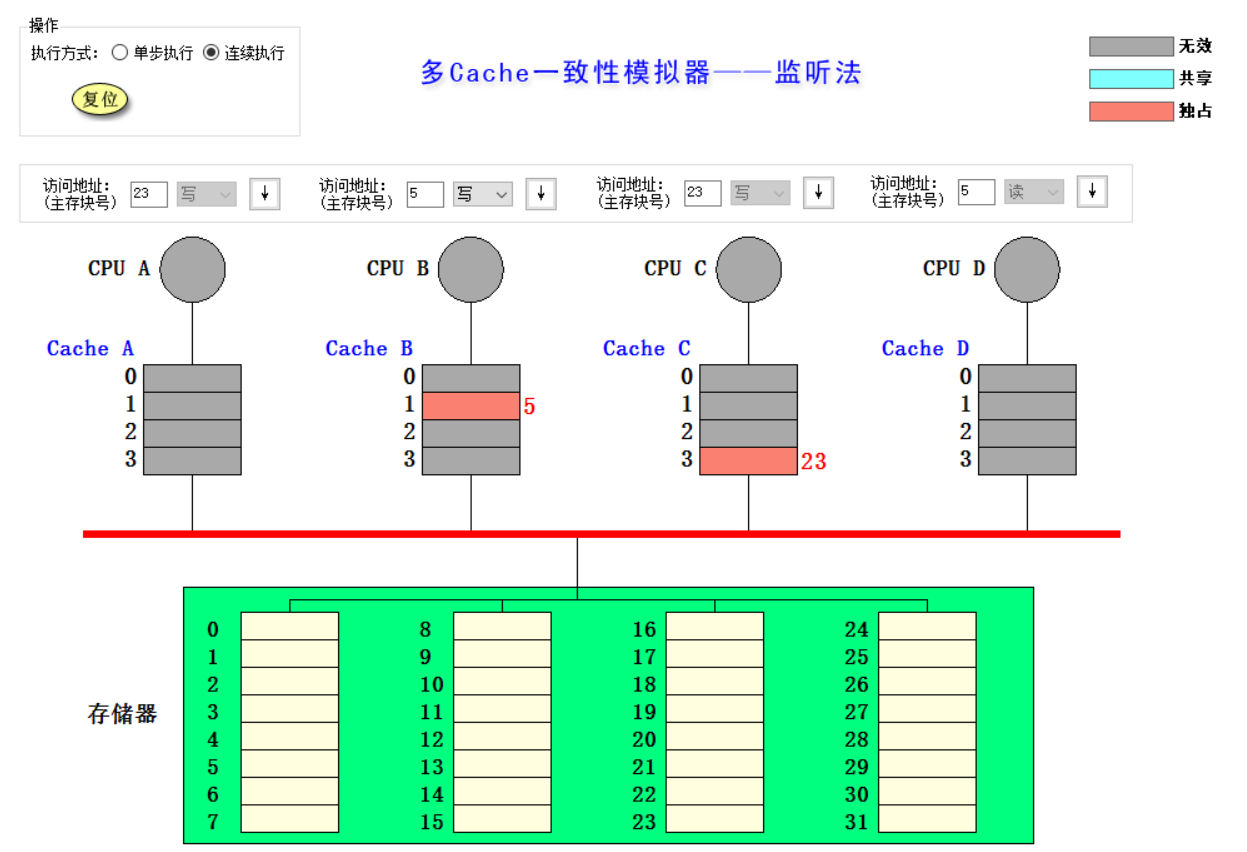
\includegraphics[scale=0.3]{jtf.png}
              \caption{执行完毕cache系统状态}
          \end{figure}
\end{enumerate}
\section{\hei 多cache一致性算法-目录法}
\begin{enumerate}
    \item 利用模拟器进行下述操作,并填写下表。
    \begin{longtable}{|l|l|l|}
        % \begin{longtable}{p{1cm}, p{1cm}, p{1cm}, p{1cm}}

        \caption{目录法}\label{tab2}

        % 表格“首页”显示内容

        \endfirsthead

        % “后续页面”表头显示内容
        \multicolumn{1}{c}{Continued}                   \\

        \endhead

        % 表格“尾页前”,表格最后显示内容

        \multicolumn{1}{c}{Continued on next page}
        \endfoot

        % 表格“尾页”,表格最后显示内容

        \endlastfoot
        \hline
        所进行的访问      & 监听协议进行的操作                                                                                                                                               & 块状态改变                                                                                                                                                               \\ \hline
        CPU A 读第6块  & \tabincell{l}{Cache A发送Read Miss到Memory A,\\Memory A传输第6块到Cache A,\\Cache A的块2从状态I转换为S}                                                                                    & \tabincell{l}{Memory A的块6,\\状态:U-\textgreater{}S,\\Presence bits:0000-\textgreater{}0001,\\共享集合\{A\}}                                                                                     \\ \hline
        CPU B 读第6块  & \tabincell{l}{Cache B发送Read Miss到Memory A,\\Memory A传输第6块到CacheB,\\Cache B的块2从状态2转为S}                                                                                      & \tabincell{l}{Memory A的块6,\\状态:S-\textgreater{}S,\\Presence bits:0001-\textgreater{}0011,\\共享集合\{A, B\}}                                                                                  \\ \hline
        CPU D 读第6块  & \tabincell{l}{Cache D发送Read Miss到Memory A,\\Memory A传输第6块到Cache D,\\Cache D的块2从状态I转为S}                                                                                      & \tabincell{l}{Memory A的块6,\\状态:S-\textgreater{}S,\\Presence bits: 0011-\textgreater{}1011,\\共享集合\{A,B,D\}}                                                                                \\ \hline
        CPU B 写第6块  & \tabincell{l}{Cache B发送Write Hit到Memory A,\\Memory A发送Invalidate(6)到Cache A,\\Cache A的块2从状态S转为I,\\Memory A发送Invalidate(6)到到Cache D,\\Cache D的块2从状态S转换到I,\\Cache B的块2从状态S转换到M}     & \tabincell{l}{Memory A到块6,\\状态:S-\textgreater{}M,\\Presence bits:1011-\textgreater{}0010,\\共享集合\{B\}}                                                                                     \\ \hline
        CPU C 读第6块  & \tabincell{l}{Cache C发送Read Miss到Memory A,\\Memory A发送Fetch(6)到Cache B,\\Cache B传输第6块到Memory A,\\Cache B的块2从状态M转为S,\\Memory A传输第6块到Cache C,\\Cache C的块2从状态I转为S}                   & \tabincell{l}{Memory A的块6,\\状态:M-\textgreater{}S,\\Presence bits:0010-\textgreater{}0110,\\共享集合:\{B,C\}}                                                                                  \\ \hline
        CPU D 写第20块 & \tabincell{l}{Cache D发送Write Miss到Memory C,\\Memory C传输第20块到Cache D,\\Cache D的块0从状态I转为M}                                                                                    & \tabincell{l}{Memory C的块20,\\状态:U-\textgreater{}M,\\Presence bits:0000-\textgreater{}1000,\\共享集合\{D\}}                                                                                    \\ \hline
        CPU A 写第20块 & \tabincell{l}{Cache A发送Write Miss到Memory C,\\Memory C发送Fetch\\\&Invalidate(20)到Cache D,\\Cache D传输第20块到Memory C,\\Cache D的块0从状态M转为I,\\Memory C传输第20块到Cache A,\\Cache A的块0从状态I转换到M}  & \tabincell{l}{Memory C的块20,\\状态:M-\textgreater{}M,\\Presence bits:1000-\textgreater{}0001,\\共享集合\{A\}}                                                                                    \\ \hline
        CPU D 写第6块  & \tabincell{l}{Cache D发送Write Miss到Memory A,\\Memory A发送Invalidate(6)到Cache B,\\Cache B的块2从状态S转为I,\\Memory A传输第6块到Cache D,\\Cache D的块2从状态I转为M}                                   & \tabincell{l}{Memory A的块6,\\状态:S-\textgreater{}M,\\Presence bits:0110-\textgreater{}1000,\\共享集合\{D\}}                                                                                     \\ \hline
        CPU A 读第12块 & \tabincell{l}{Cache A发送Write Back到Memory C,\\Cache A的块0从状态M转为I,\\Cache A发送Read Miss到Memory B,\\Memory B传输第12块到Cache A,\\Cache A的块0从状态I转为S}                                      & \tabincell{l}{Memory C的块20,\\状态:M-\textgreater{}U,\\Presence bits:0001-\textgreater{}0000,\\共享集合\{\};\\Memory B的块12,\\状态:U-\textgreater{}S,\\Presence bits:0000-\textgreater{}0001,\\共享集合:\{A\}}  \\ \hline
        
        \end{longtable}
    \item 请截图,展示执行完以上操作后整个cache系统的状态。
    \par \begin{figure}[H]
        \centering
        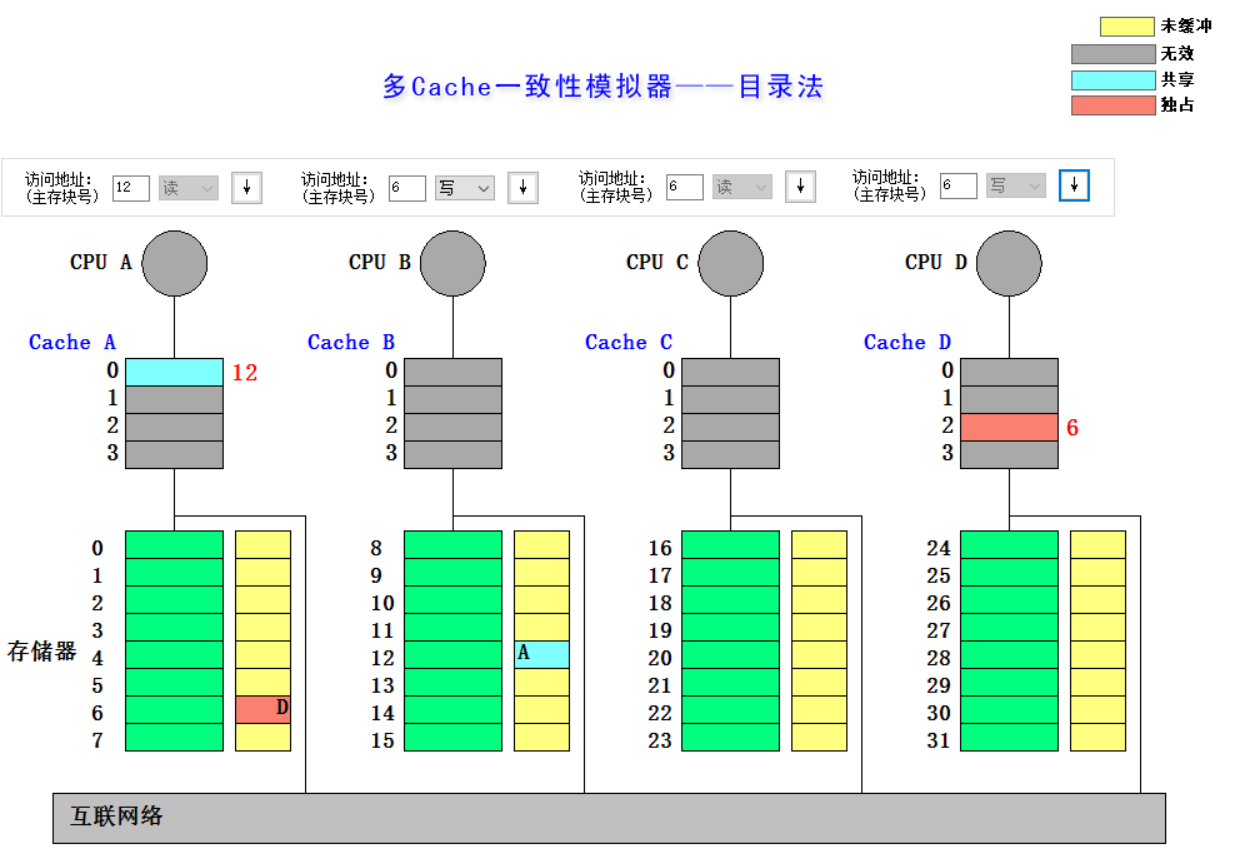
\includegraphics[scale=0.3]{mlf.png}
        \caption{执行完毕cache系统状态}
    \end{figure}
\end{enumerate}
\section{\hei 综合问答}
\begin{enumerate}
    \item 目录法和监听法分别是集中式和基于总线,两者优劣是什么?(言之有理即可)
    \par 监听法:
    \par \quad 优点:保证了Cache的一致性,实现了写互斥和写串行
    \par \quad 缺点:\begin{itemize}
        \item 扩展性差,总线上能够连接的处理器数目有限
        \item 存在总线竞争问题
        \item 总线的带宽会带来一些限制
        \item 在非总线和或环形网络上监听困难
        \item 总线事务多,通信开销大
    \end{itemize}
    \par 目录法:
    \par \quad 优点:\begin{itemize}
        \item 拓展性强,可以连接的处理器数目更多 
        \item 降低了对于总线带宽的占用
        \item 可以有效地适应交换网络进行通信
    \end{itemize}
    \par \quad 缺点:\begin{itemize}
        \item 需要额外的空间来存储Presence Bits,当处理器数目较多的时候会有很大的存储开销
        \item 总线竞争
        \item 存储器接口通信压力大,存储器速度成为限制
    \end{itemize}
    \item Tomasulo算法相比Score Board算法有什么异同?(简要回答两点:1.分别解决了什么相关,2.分别是分布式还是集中式)(参考第五版教材)
    \par Tomasulo算法
    \par \quad 解决的相关:
    \begin{itemize}
        \item WAR相关:使用RS的寄存器或指向RS的指针代替指令中的寄存器-寄存器重命名
        \item WAW相关:使用RS中的寄存器值或指向RS的指针代替指令中的寄存器
        \item RAW相关:检测到寄存器就绪即没有冲突再读取操作数,进入执行阶段
        \item 结构相关:有结构冲突不发射
        \item 结果Forward:从FU广播结果到RS和寄存器
    \end{itemize}
    \par \quad 特点:分布式;指令状态、相关控制和操作数缓存分布在各个部件中(保留站)
    \par Score Board算法
    \begin{itemize}
        \item WAR相关:对操作排队,仅在读操作数阶段读寄存器
        \item WAW相关:检测到相关后,停止发射前一条指令,直到前一条指令完成
        \item RAW相关:检测到没有冲突(寄存器就绪)再读取操作数,进入执行阶段
        \item 结构相关:有结构相关不发射
        \item 结果Forward:写回寄存器接触等待
    \end{itemize}

    \item Tomasulo算法是如何解决结构、RAW、WAR和WAW相关的?(参考第五版教材)
    \par 结构相关:有结构冲突不发射
    \par RAW相关:检测到没有冲突,即存储器就绪再读取操作操作数,进入执行阶段
    \par WAW相关:使用RS中的寄存器值或指向RS的指针代替指令中的寄存器-寄存器重命名
    \par WAR相关:使用RS中的寄存器值或指向RS的指针代替指令中的寄存器-寄存器重命名
\end{enumerate}
\end{document}